\scanpage{29}
% archive sheet number: 35

\mspage{16}

% top centre
$V$ plan \unsure{vect|vect.} $/k$, $n$ entier $\geq\deleted{\unsure{3|2}}1$

% top, below first line
\uline{Théorème} $u_*=(u_i)_{i\in\mathbb Z/n\mathbb Z}\in{\unsure{V|k}}^{\mathbb Z/n\mathbb Z}$, les $u_i\ne0$

% upper quarter
\[
 N(u_*)=\bigl\{(\lambda_i)\in k^{\mathbb Z/n\mathbb Z}\mid
 \deleted{\sum}\lambda_{\unsure{i|i-1}}u_{i-1}\unsure{-|+}\lambda_i(u_i+u_{i+1})+
 \lambda_{i+1}u_{i-2}=0\qquad\forall i\in\mathbb Z/n\mathbb Z\bigr\}
\]

% below definition
Soit $H_i\subset k^{\mathbb Z/n\mathbb Z}$ hyperplan coord. $i$ ème. On est alors dans les cas \unsure{mutuelt|mutuelmt} exclusifs

% left opposite a
% slanted
\margin{``\uline{Cas général}''}

% upper middle, case a circled
\textcircled{a} $\dim N(u_*)=0$ i.e. $N(u_*)=0$ [i.e., si $\sum u_i=0$, l'application \inserted{can} $\varphi:\unsure{X|\mathcal X}(W)\longrightarrow(\det V)^{\mathbb Z/n\mathbb Z}$ est \uline{lisse} en $u_*$]

% middle, case b circled
\textcircled{b} \deleted{$\dim N(u_*)=1$, \unsure{et|si} \inserted{dim} $N(u_*)=1$ et}

% middle, below cancelled line
\[
 N(u_*)\not\subset\bigcup H_i\quad(\Longrightarrow\ \dim N(u_*)\in\{1,2\})
\]

% left opposite b1
% slanted
\margin{``Cas spécial I''}

% middle, first subcase circled
\[
 \text{\textcircled{$b_1$}}\qquad \dim N(u_*)=1
\]

% left opposite b2
% slanted
\margin{``\uline{Cas hyperspécial}''}

% middle, second subcase circled
\[
 \text{\textcircled{$b_2$}}\qquad \dim N(u_*)=2\quad\Longleftrightarrow
 \left\{\begin{aligned}u_i&=u_{i+3}\\u_0+u_1+u_2&=0\end{aligned}\right.
\]

% left opposite c
% slanted
\margin{``Cas spécial II''}

% below middle, case c and linked outlines
\figure{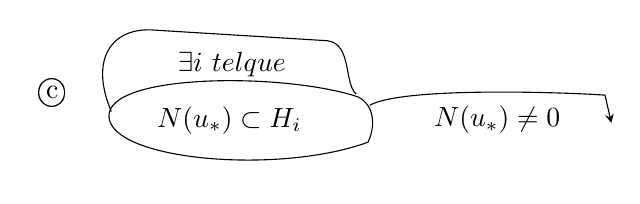
\begin{tikzpicture}[x=1cm,y=.72cm,>=stealth]
\node at (-2.25,-.16) {\textcircled{c}};
\node at (.03,.4) {$\exists i\ \text{tel que}$};
\node at (0,-.58) {$N(u_*)\subset H_i$};
\node at (3.4,-.57) {$N(u_*)\ne0$};
\draw (-1.5,-.42) .. controls (-1.78,.50) and (-1.50,1.05) .. (-.99,1.02)
 -- (1.24,.83) .. controls (1.56,.78) and (1.45,.08) .. (1.61,-.11);
\draw (1.63,-.16) .. controls (.7,.27) and (-1.56,.26) .. (-1.53,-.51)
 .. controls (-1.50,-1.28) and (.62,-1.54) .. (1.76,-.96)
 .. controls (1.86,-.67) and (1.84,-.30) .. (1.63,-.16);
\draw[->] (1.78,-.31) .. controls (2.20,.02) and (4.25,-.08) .. (4.77,-.13)
 -- (4.85,-.62);
\end{tikzpicture}}

% lower third, consequence of c
($\Rightarrow\dim N(u_*)=1$, si $\underset{\ne0}{\lambda}=(\lambda_i)\in N(u_*)$, \deleted{\unsure{donc|avec}} (\unsure{disons}) $\lambda_{i_0}=0$, les \deleted{$\unsure{\lambda|i}$} $i$ tels que $\lambda_i=0$ sont ceux pour lesquels $s_i=s_{i_0}$ (i.e. $u_{i_0}\mathbin{\text{---}}+u_{i-1}=0$)

% lower left, diagonal, three numbered conditions
% slanted
\margin{$\exists O\in E$, droite $\Delta\in E$ \unsure{passant par} $O$, tels que $\forall i$ tels que \unsure{1°)} \deleted{$\lambda_i\ne0$} $u_{i-1}$ \deleted{$\unsure{u_i=0|u_{0i}=0}$} $//\Delta$ et \deleted{$\unsure{u_{i-1}|u_i}$} $u_i\unsure{\longrightarrow|-}//u_{0\unsure{i|2}}$, on \unsure{aura|avant} 2°) $\exists i$, \unsure{un} $s_i\ne0$ 3°) \unsure{du moins} \illegible{2} \unsure{les} $(s_i)$. $\Longleftrightarrow$}

% foot, condition and normalization
Pour qu'on soit dans le cas c, \inserted{où $\lambda_0=0$,} il f et s \deleted{\unsure{que}} que

% foot, conditions a and b
\[
 \begin{aligned}
 &\mathrm a)\quad \sum u_i=0\\
 &\mathrm b)\quad \forall\deleted{\unsure{i|0}}\,1\leq i\leq n-1,\ \text{on ait}\\
 &\hspace{6em} u_{i-1}\,u_i\ //\ u_1\,u_{0i}
 \end{aligned}
\]

% bottom line
et si \inserted{on normalise} $\lambda_1=1$, on aura $\lambda_i$ défini par $u_1u_{0i}=\lambda_i u_i u_{i-1}$\unsure{.}
